\section{Objectives}
\label{sec-objectives}
The main goal in this TFG is to detect seizures from the dataset CHB-MIT. To fulfil the objective an architecture has been created working within a pipeline of events. Starting by finding the best data analysis and processing method before feeding it to the deep learning algorithms. There are many sub-objectives to be completed to obtain good results from this architecture and also, it’s modular for further expansion and studies. The main strategy of the scripts execute in sequence:
\\
\begin{figure}[h!]
    \caption{Scheme of data processing }
    \centering
    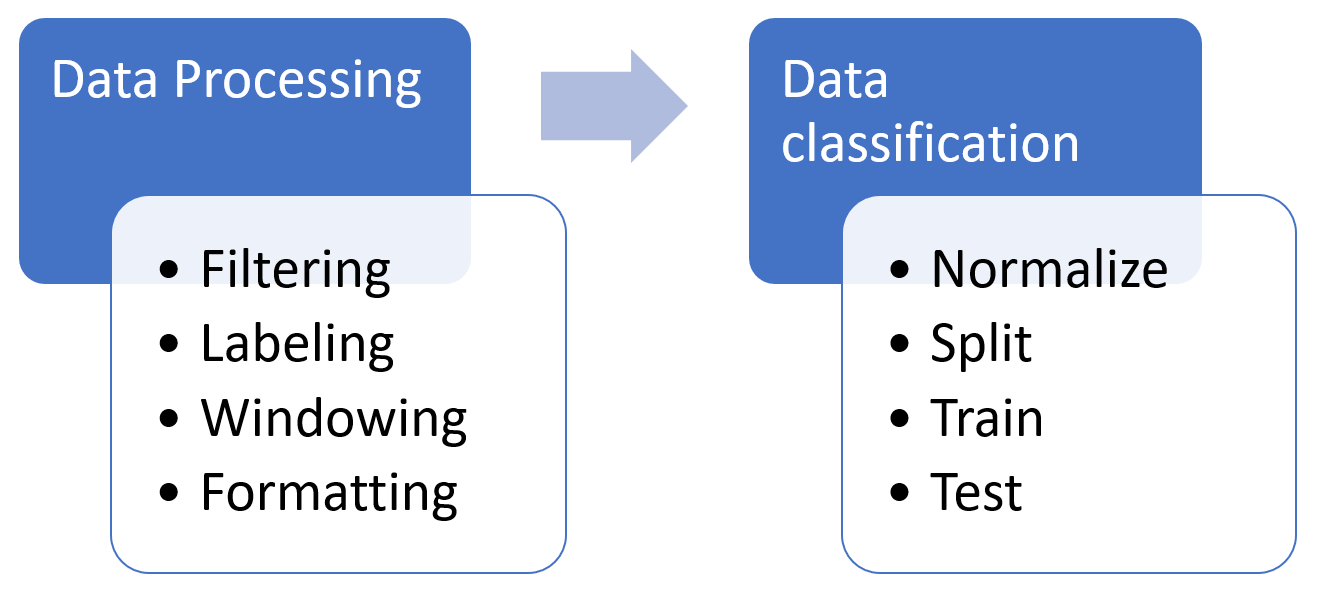
\includegraphics[width=0.5\textwidth]{img/pipeline.png}
\end{figure}
\\
To fulfil the objectives is crucial to define smaller objectives to make work easier. Within the first objective there are several important parts: 
\\
\begin{itemize}

    \item Raw data must be readable, as the data base CHB-MIT\cite{goldberger2000physiobank} is in European Data Format (EDF), a standard file format designed for exchange and storage of medical time series, so all files in the dataset are “.edf”. A script has been programmed to save .edf files into .parquet format.
    \item Setting different functions to filter data making sure data fits certain constraints to obtain better results when training the model.
    \item Get the labelling data, to have a ground truth from the recorded data. This part is essential to understand if the model works as expected.
    \item Define different functions to define how data enters the model to be trained. There are many ways information can be extracted from data. 
    \item Each model needs to be configured to accept the dimensionality of the data fed to it.
    \item Work different models to choose what models give better answers form input data.
    \item After all the models results, an overview is done to understand the results and conclude the best way to treat this database, for further investigation.

\end{itemize}